\begin{frame}{Agentic RAG với LangGraph 1}

\begin{figure}[H]
\centering
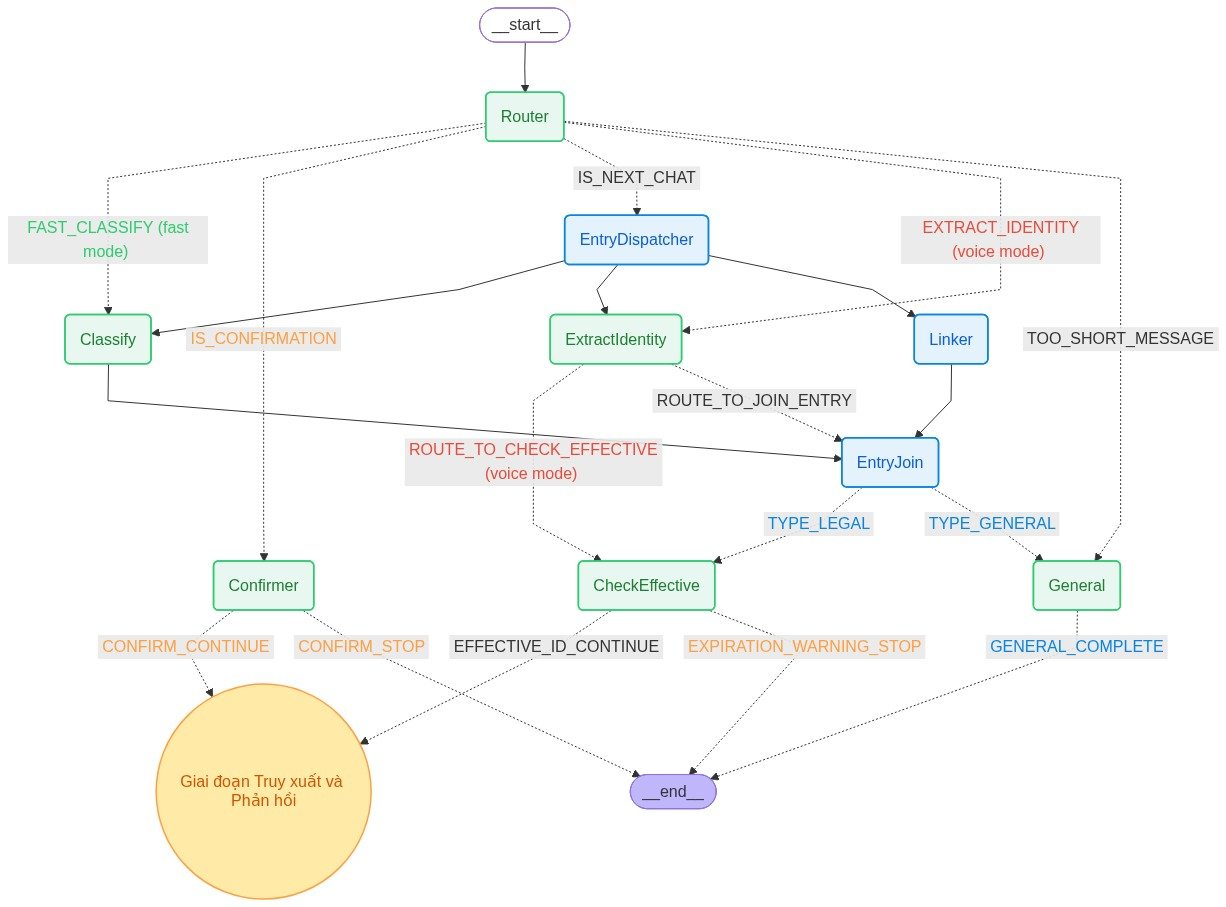
\includegraphics[width=\linewidth,height=0.74\textheight,keepaspectratio]{pictures/LangGraph/LangGraph1.png}
\caption{Sơ đồ LangGraph của dự án}
\end{figure}

\note{
Ở giai đoạn đầu
Có các node thực hiện các công việc đồng thời
Phân loại
Trích xuất số hiệu văn bản
Tìm thông tin url nếu có đề cập
Nếu câu hỏi thuộc loại chung hoặc quá ngắn thì ai thực hiện trả lời chung giúp tiết kiệm tài nguyên
Nếu có số hiệu văn bản thì sẽ tra cứu hiệu lực
Nếu đã hết hiệu lực thì tạm dừng ngay
Nếu hết hiệu lực 1 phần tạm dừng và hỏi xác nhận
Nếu còn hiệu lực hoặc có xác nhận từ người dùng thì sẽ đến bước giai đoạn truy xuất dữ liệu

}
\end{frame}
